% --------------------------------------------------------------
% This is all preamble stuff that you don't have to worry about.
% Head down to where it says "Start here"
% --------------------------------------------------------------
 
\documentclass[12pt]{article}
 
\usepackage[margin=1in]{geometry} 
\usepackage{amsmath,amsthm,amssymb}
\usepackage{graphicx}
\usepackage{soul}
\usepackage[utf8]{inputenc}
\usepackage{comment}

\usepackage{url}
\usepackage{hyperref}
\hypersetup{
    colorlinks=true,
    linkcolor=blue,
    filecolor=magenta,      
    urlcolor=cyan,
    }
\newcommand{\N}{\mathbb{N}}
\newcommand{\Z}{\mathbb{Z}}

\usepackage{xcolor}
\newcommand{\red}[1]{{\color{red}#1}}
 
\newenvironment{theorem}[2][Theorem]{\begin{trivlist}
\item[\hskip \labelsep {\bfseries #1}\hskip \labelsep {\bfseries #2.}]}{\end{trivlist}}
\newenvironment{lemma}[2][Lemma]{\begin{trivlist}
\item[\hskip \labelsep {\bfseries #1}\hskip \labelsep {\bfseries #2.}]}{\end{trivlist}}
\newenvironment{exercise}[2][Exercise]{\begin{trivlist}
\item[\hskip \labelsep {\bfseries #1}\hskip \labelsep {\bfseries #2.}]}{\end{trivlist}}
\newenvironment{reflection}[2][Reflection]{\begin{trivlist}
\item[\hskip \labelsep {\bfseries #1}\hskip \labelsep {\bfseries #2.}]}{\end{trivlist}}
\newenvironment{proposition}[2][Proposition]{\begin{trivlist}
\item[\hskip \labelsep {\bfseries #1}\hskip \labelsep {\bfseries #2.}]}{\end{trivlist}}
\newenvironment{corollary}[2][Corollary]{\begin{trivlist}
\item[\hskip \labelsep {\bfseries #1}\hskip \labelsep {\bfseries #2.}]}{\end{trivlist}}
 
\begin{document}
 
% --------------------------------------------------------------
%                         Start here
% --------------------------------------------------------------
 
%\renewcommand{\qedsymbol}{\filledbox}
 
\title{Kaggle Competition 1 IFT 6390/3395}
 
\maketitle

\section{Introduction}
\label{sec:intro}

For this project, you will take part in a Kaggle competition about detection of handwritten digits. The goal is to design a machine learning algorithm that can automatically classify images. Figure \ref{fig:my_label} shows an example image from the training set. All the images (including held out test samples) are of dimension $56\times28$. The class for a image is denoted by the sum of digits in the image. For example, the class of image in figure \ref{fig:my_label} is 10. We have generated this dataset from the popular \href{http://yann.lecun.com/exdb/mnist/}{MNIST} dataset. The training and held-out test set for this data consists of 50,000 samples and 10,000 samples respectively.
\begin{figure}[h]
    \centering
    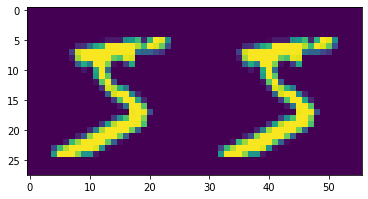
\includegraphics[width=0.5\linewidth]{figures/img1.png} 
    
    \caption{Example image from the training set}
    \label{fig:my_label}
\end{figure}
You are required to implement and train several classification algorithms based on the dataset provided. The evaluation will be based on the performance on the held out test set and a written report.

The competition, including the data, is available here: 

\begin{center}
\href{https://www.kaggle.com/t/0d0b1c033ece47ffa1dbc8bd374689ae}{https://www.kaggle.com/t/0d0b1c033ece47ffa1dbc8bd374689ae}
\end{center}

\section{Important dates and information}
\label{sec:dates}

Please take into consideration the following important deadlines:
 
% TODO: confirm dates
\begin{itemize}
 \item \textbf{October 5th 23:59} Competition released
 \item \textbf{October 12th 23:59} Deadline to enter the competition on Kaggle.
 \item \textbf{October 26th 23:59} Competition ends. No more Kaggle submissions are allowed.
 \item \textbf{November 3rd 23:59} Reports and code are due on Gradescope.
\end{itemize}
 
\textbf{Note on sharing and plagiarism}:
You are allowed to discuss general techniques with other teams. You are NOT allowed to share any of your code. This behavior constitutes plagiarism and it is very easy to detect. All teams involved in sharing code will receive a grade of 0 in the data competition.”

\section{Join the competition}

\textbf{IFT6390} students must do the competition alone (1-person team) (\textbf{IFT3395} students will participate in teams of 2 or 3).


\subsection{Kaggle Team formation (IFT3395 students only)}

To form a team:
\begin{itemize}
\item Enter the competition and create a Kaggle account if you are not registered yet by following the link: \href{https://www.kaggle.com/t/0d0b1c033ece47ffa1dbc8bd374689ae}{https://www.kaggle.com/t/0d0b1c033ece47ffa1dbc8bd374689ae}
\item In the ``Invite Others" section, enter your teammates’ names, or team name.
\item Your teammate has the option to accept your merge.
\item Fill out the google form \url{https://forms.gle/Jrscpc5p6ee3x9Vw7} with your team information by \textbf{October 12th at 23:59}. Any teams not registered or registered late will not be graded.

\end{itemize}
\textbf{Important note:} The maximum amount of submissions per day and per team is 2. Any team whose individual members have a submission count larger than what is allowed up to-date will be unable to form a team. Example: Today is the first day of competition. A,B,C are three teammates who haven’t formed a team yet.

\begin{itemize}
    \item A submitted 0 times.
    \item B submitted 2 times.
    \item C submitted 1 time.
\end{itemize}

Because the maximum amount of submissions is 2 per team per day, the total possible submissions for a team is 2. However, the cumulative submission count for A,B,C is 3. Therefore, they will be unable to form a team. They will need to wait for tomorrow, and not submit any submissions for the next day.

You can start submitting solutions before you form a team, as long as you are careful about the above limitation when forming teams. 


\section{Baselines}
\label{sec:baselines}

% TODO: add baselines to Kaggle competition
We ask you to build a \textbf{logistic regression} classifier and beat the baselines highlighted in the leaderboard. These baselines are:

\begin{itemize}
    \item a dummy classifier that simply predicts the most frequent class in the training set.
    \item a logistic regression classifier.
    \item the TA's best baseline.
\end{itemize}

To participate in the competition, you must provide a list of predicted outputs for the instances on the Kaggle website. You can submit 2 predictions per day over the course of the competition, so we suggest you start early, allowing yourself enough time to submit multiple times and get a sense of how well you are doing.

For each of the 3 baselines that you beat, you get extra points.

Your logistic regression classifier must be implemented from scratch. Apart from standard Python libraries, the only libraries allowed are \texttt{numpy}, sparse matrices from scipy (\texttt{scipy.sparse}), and \texttt{pandas}.

\section{Other models}
 
You must try at least \textbf{1 other model} besides logistic regression, and compare their performances. You are encouraged to implement techniques studied during the course, and look up for other ways to solve this task. Here are a few ideas:

\begin{itemize}
    \item Support Vector Machines
    \item Na\"ive Bayes
    \item Random Forests 
    \item Hand-crafted features that take into account the nature of the data
\end{itemize}

The goal is to design the best performing method as measured by submitting predictions for the test set on Kaggle. Your final performance on Kaggle will count as a criterion for evaluation (see Section \ref{sec:report}). If a tested model does not perform well, you can still add it in your report and explain why you think it is not appropriate for this task. This kind of discussion is an important feature that we will be using to evaluate your final competition report.

For this part, you are free to use any library of your choice.

\section{Report}
\label{sec:report}

In addition to your methods, you must write up a report that details the pre-processing, validation, algorithmic, and optimization techniques, as well as providing results that help you compare different methods/models.

The report should contain the following sections and elements:

\begin{itemize}
  \item Project title
  \item Full name, student number and Kaggle username.
  \item Introduction: briefly describe the problem and summarize your approach and results.
  \item Feature Design: Describe and justify your pre-processing methods, and how you designed and selected your features.
  \item Algorithms: give an overview of the learning algorithms used without going into too much detail, unless necessary to understand other details.
  \item Methodology: include any decisions about training/validation split, regularization strategies, any optimization tricks, choice of hyper-parameters, etc.
  \item Results: present a detailed analysis of your results, including graphs and tables as appropriate. This analysis should be broader than just the Kaggle result: include a short comparison of the most important hyper-parameters and all methods (at least 2) you implemented.
  \item Discussion: discuss the pros/cons of your approach and methodology and suggest ideas for improvement.
  \item  Statement of Contributions. add the following statement: ``I hereby state that all the work presented in this report is that of the author''.
  \item References: very important if you use ideas and methods that you found in some paper or online; it is a matter of academic integrity.
  \item Appendix (optional). Here you can include additional results, more details of the methods, etc.
  \end{itemize}
  
You will lose points for not following these guidelines. \textbf{The main text of the report should not exceed 6 pages.} References and appendix can be in excess of the 6 pages. 
%The format should
%be single column, 10pt font, min. 1 margins. You can use the standard
%IEEE conference format, e.g. https://www.ieee.org/conferences
%events/ conferences/publishing/templates.html

% TODO: confirm data
Your must submit your report and your code on Gradescope before \textbf{November 3rd 23:59}.

\subsection*{Submission Instructions}
 
\begin{itemize}
\item You must submit the code developed during the project.
The code must be well-documented.
The code should include a README file containing instructions on
how to run the code.
\item The prediction file containing your predictions on the test set must be submitted online at the Kaggle website.
\item  The report in pdf format~(written according to the general layout described above) and the code should be uploaded on Gradescope.
\end{itemize}


\section{Evaluation Criteria}


Marks will be attributed based on the following criteria:

\begin{enumerate}
    \item You will be assigned points for each one of the 3 baselines that you beat.
    \item You will be assigned points depending on your final performance at the end of the competition, given by your ranking in the private leaderboard.
    \item You will be assigned points depending on the quality and technical soundness of your final report (see above).
\end{enumerate}

% \subsection*{Evaluation of the report}

% For the written report, the evaluation criteria include:
% \begin{itemize}
% \item Technical soundness of the methodology (pre-processing, feature selection,
% validation, algorithms, optimization).
% \item Technical correctness of the description of the algorithms (may be
% validated with the submitted code).
% \item Meaningful analysis of final and intermediate results.
% \item Clarity of descriptions, plots, figures, tables.
% \item Organization and writing. Please use a spell-checker and do not underestimate
% the power of a well-written report!!
% \end{itemize}
% Do note that the grading of the report will place emphasis on the quality
% of the implemented classifiers as well as the rationale
% behind the pre-processing and optimization techniques. The code should be
% clear enough to reflect the logic articulated in the report. We are looking
% for a combination of insight and clarity when grading the reports.

\end{document}
